\section{The Quantum Approximate Optimization Algorithm (QAOA)}
The Quantum Approximate Optimization Algorithm (QAOA) was first introduced in 2014 by Fahri, Goldstone, and Gutmann \cite{farhiQAOA}. QAOA is a VQA that generates approximate solutions for combinatorial optimization problems and is said to be suitable for running on near-term devices, due to its shallow circuit depth. QAOA is a trotterized version of QAA, designed to iteratively apply alternating unitaries until the best approximation is found \cite{farhiQAOA}. The unitaries consist of a cost and a mixer where the cost is what the problem is encoded into, and the mixer is a simpler Hamiltonian for which the ground state is known \cite{review2024}. In contrast to QAA, QAOA has a feature in which as the parameter p increases, the approximation improves \cite{farhiQAOA}. 

MaxCut is a well-known combinatorial optimization problem that is often used to illustrate QAOA. This is due to its complexity (NP-hard) and its extensive research in classical algorithms. Its cost function is also easily translatable to Hamiltonians, making it a great candidate to demonstrate QAOA's capabilities. This is why the following explanation of QAOA will be to solve the MaxCut problem. The algorithm has the following steps:

1. Define a cost Hamiltonian $H_C$ that encodes the problem and construct the operator $U_C$. The cost function can be transformed to the cost Hamiltonian as such \cite{review2024}:
\begin{equation} 
        \hat{H}_C \ket{x} = C(x) \ket{x}
    \end{equation}

For MaxCut, we have already defined the cost function in (2). The Hamiltonian $H_C$ and operator $U_C$ can be written as:

\begin{equation} 
    H_C = \sum_{i,j=0}^{n} \frac{w_{ij}}{2} (\mathbb{I} - \sigma_i^Z \sigma_j^Z)
\end{equation}

\begin{equation} 
        U_C = e^{-i \gamma H_C}
\end{equation}

2. Construct a second Hamiltonian and operator, $H_M$, which we call the mixer. This is typically the mixer Hamiltonian used for MaxCut \cite{farhiQAOA}:

\begin{equation} 
        H_M =  \sum_{i=0}^{n} \sigma_i^X   \hspace{+8mm}
        U_M = e^{-i \beta H_B}
    \end{equation}

where $\sigma^X$ is the Pauli-X operator \cite{farhiQAOA}. Recall that the exponential of a single-qubit unitary can be expressed as a rotation, so we can write $U_M$ as \cite{classBook}: 
\begin{equation} 
    U_M(\beta) = \prod_{i=1}^{n} R_{X_i}(2 \beta) 
\end{equation}

\begin{figure*}[ht]
    \centering
    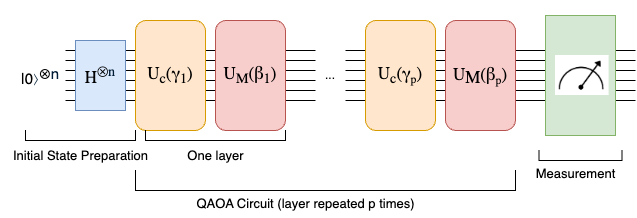
\includegraphics[width=0.75\linewidth]{images/QAOACircuit.drawio.png}
    \caption{Figure adapted from \cite{review2024}. Shows an example QAOA circuit with the initial state being prepared as $\ket{++..+}$}
    \label{fig:Figure 3}
\end{figure*}

3. Initialize the state in the highest energy state of the mixer, $H_M$ \cite{review2024}:

\begin{equation} 
    \ket{\psi_0} = \ket{+}^{\otimes n} = \frac{1}{\sqrt{2^n}} \sum_{x=0}^{2^n -1} \ket{x}
\end{equation}

4. Construct the QAOA circuit. Once the state is initialized, the circuit is created by repeating the QAOA layer p times \cite{farhiQAOA} (see Fig. 3). The QAOA layer is defined as the $U_C$ operator followed by the $U_M$ operator \cite{farhiQAOA}. There are also 2p parameters that need to be defined: $\gamma_{1-p}$ and $\beta_{1-p}$ such that $\gamma \in [0,2*\pi)$ and $\beta \in [0,\pi)$ \cite{review2024}. The circuit is defined as \cite{farhiQAOA}:

\begin{equation} 
    \ket{\psi} = \hat{U}_C(\gamma_p) \hat{U}_M(\beta_p) ... \hat{U}_C(\gamma_1) \hat{U}_M(\beta_1)\ket{\psi_0}
\end{equation}

5. Next, find the expectation value of $H_C$ in this state $\ket{\psi}$, which represents the cost obtained for the problem \cite{qaoaNearTerm}:

\begin{equation} 
    F_p(\gamma, \beta) = \braket{\psi_p(\gamma, \beta)|H_C|\psi_p(\gamma, \beta)}
\end{equation}

6. A classical computer is then used to optimize the parameters $\gamma$ and $\beta$ to maximize the expectation value (cost) \cite{qaoaNearTerm}. This optimization can be performed in a variety of ways, such as gradient descent optimization \cite{qaoaNearTerm}. Once the expectation value is maximized, the quality of the approximation is calculated using the approximation ratio (equation 5).

\subsection{Application to QAA}
Fahri et al. also discuss the connection of QAOA to QAA (see section 2.2.2) \cite{farhiQAOA}. QAOA is focused on finding an approximate solution to the problem, while the Quantum Adiabatic Algorithm (QAA) is designed to find the optimal solution if the Hamiltonian is evolved slowly enough (if the runtime is long enough). Consider the adiabatic evolution with runtime T: 
\begin{equation} 
    H(t) = \frac{t}{T}H_C + (1- \frac{t}{T})H_M
\end{equation}

Where $H_M$ is our mixer Hamiltonian, which defines our initial state as its highest energy state, $\ket{+}$ and $H_C$ is our cost Hamiltonian. A Trotterized approximation to this time evolution corresponds to a layer of QAOA. So, according to the adiabatic theorem, if p is large enough ($p \rightarrow \infty$), QAOA would produce the optimal solution. 